\section{Repository Structure}\label{sec_Respository_Structure}
\begin{comment}
% Vorlage
\begin{figure}[h]
	\centering
	\resizebox{0.2\textwidth}{!}{% Faktor zum Skalieren
		\begin{forest}
			for tree={
				font=\sffamily,
				grow'=0,
				folder indent=0.9em,
				folder icons,
				edge=densely dotted
			}
			[Application
			[bin]
			[conf
			[.yaml, is file]
			]
			[data]
			[doc
			[scipt-1.me, is file]	
			[$\quad\vdots$, is file] % gepunktete Linien werden so unterdrückt, Format wird aber nicht eingehalten.
			[scipt-$n$.me, is file]
			]
			[log
			[.txt/.json, is file]
			]
			[script/
			[script 1
			[$\_\_$init$\_\_$.py, is file]
			[Module.py, is file]
			]
			[$\quad\vdots$, is file] % gepunktete Linien werden so unterdrückt, Format wird aber nicht eingehalten.
			[scipt $n$
			[$\_\_$init$\_\_$.py, is file]
			[Module.py, is file]
			]
			[$\_\_$init$\_\_$.py, is file]
			[main.py, is file]
			]
			[tests]
			[Read.me, is file]
			[.gitignore, is file]
			]
		\end{forest}
	}%
	\caption{Struktur für Ordner im Repository, \href{https://tex.stackexchange.com/questions/5073/making-a-simple-directory-tree}{Verweis}}
	\label{fig: Struktur für Ordner im Repository}
\end{figure}
\end{comment}

Um eine \textit{kontinurierliche Integration} von neuen Code-Bestandteilen, Feature, Bug-Fixes zu gewähren, wird das im Folgenden die folgende Struktur etabliert.
\begin{figure}[h]
	\centering
	\resizebox{0.2\textwidth}{!}{% Faktor zum Skalieren
		\begin{forest}
			for tree={
				font=\sffamily,
				grow'=0,
				folder indent=0.9em,
				folder icons,
				edge=densely dotted
			}
			[Application
			[..., is file]
			[test
				[Unit1$\_$test.py, is file]
				[Unit2$\_$test.py, is file]
			]
			[log/]
			[scr/
				[conf
					[$\_\_$init$\_\_$.py, is file]
					[config.py, is file]
				]
				[slapping
					[$\_\_$init$\_\_$.py, is file]
					[Upload.py, is file]
					[Download.py, is file]
				]
			]
			[requirements.txt, is file]
			[requirements$\_$conda.yml, is file]
			[requirements$\_$test.txt, is file]
			[requirements$\_$conda$\_$test.yml, is file]
			[main.py, is file]
			[LICENSE, is file]
			[Readme.md, is file]
			[..., is file]
			]
		\end{forest}
	}%
	\caption{Bsp.: Modul Aufbau unter \textit{src}}
\end{figure}

\begin{description}
	\item[scr] Module für die Applikation werden hier hinterlegt. Zu jedem Modul wird eine leere Datei $\_\_$init$\_\_$.py mit gespeichert. Diese lässt den Komplierer nachvollziehen, dass es sich hierbei um ein Modul handelt.	
	\item[tests] Unit Tests werden hier gespeichert. Jedes Skript welches mit dem Suffix $test$ versehen wird, ist ein \textit{Unit Modul}: $<Unit Modul>\_test$. Jeder Test in einem Modul wird als Funktion mit dem Prefix $test\_$ versehen: $test\_<Unit Funktion>$.
	\item[log, conf] Log-Dateien und Variablen-Konfigurations-Dateien wird hier hinterlegt.
	\item[Allgemeine Konfigurationen] Konfigurationen bezüglich des Repository und der Tests werden in Hauptverzeichnis abgelegt.
\end{description}
Weiter Bestandteile für Build Prozesses sind hier nicht enthalten. Die Konfigurationen für die Testmodule und Setuptools wird im Hauptverzeichnis hinterlegt.

\section{Virtual Environment}
\subsection{Allgemein}
Eine \gls{VEN} ist eine Ordner-Verzeichnis, in welchen Bibliothek-Pakete (aka. Pakete) abgelegt werden. Jedes Paket ist zu einer jeweiligen Version gespeichert. Dies stelle sicher zum einen sicher, dass die benötigten Pakete für ein Programm in einem Container liegen. Dieser kann einzeln separat von jeweiligen Updates an den Paketen selbst verwaltet werden. Die Informationen über diesen Container werden in Form einer \textit{requirment} Datei mit im Repository hinterlegt. Diese Information erlaubt, das testen und Ausführen des Programmes auf anderen Rechner oder Server. Die genaue Abhängikeit zu den spezifischen Versionen wird so übermittelt, damit eine genauer Kopie des Containers erstellt wird.\\

Drei Werkzeuge für die Aufsetzung von \gls{VEN} für die Python Entwicklung sind in \textit{Visual Studio} verfügbar. \footnote{
	\href{Quelle}{https://code.visualstudio.com/docs/python/environments},
	\href{Conda VE in VStudio}{https://youtu.be/Wuuiga0wKdQ}
}
\begin{description}
	\item[pip] ist ein Paket Manager für Python Pakete. Pakete können von einem öffentlichen Index \textit{PyPI} installiert werden.
	\item[venv] erstellt \gls{VEN} für Entwicklungen in Python.
	\item[conda] ist ein Paket Manager \textbf{und} eine Verwaltungssystem für \gls{VEN}. 
\end{description}

\subsection{conda}

\gls{g_conda} wird über Anaconda und Miniconda installiert. \footnote{
	Es gibt die Empfehlung für Data Science Projekte dies zu nutzen.
}
Ebenso kann pip über \gls{g_conda} installiert werden, sodass auch Pakete in einem \gls{VEN} über \gls{g_conda} installiert werden. Dies erlaubt Pakete über \gls{g_conda} und \gls{g_pip} in einer \gls{g_conda} \gls{VEN} zu installieren.\footnote{
	\href{Quelle}{https://stackoverflow.com/questions/20994716/what-is-the-difference-between-pip-and-conda}
}

\subsubsection{Create VEU} 
Eine neue \gls{VEN} kann über zwei Wege erstellt werden
\begin{description}
	\item[Terminal] Über das Terminal wird der Befehl
	\begin{lstlisting}[style=CMD]
	conda env create -f conda_requirement.yml
	\end{lstlisting} eingegeben. 
	\item[Navigator] Über den Navigator kann in der \gls{GUI} eine neue Umgebung angelegt werden.
\end{description}

Zum Punkt ein. Um \textbf{conda} direkt über das Terminal zu nutzen, muss die Shell aufgerufen werden. Dies kann zum einen über den \textbf{Anaconda Navigator} passieren oder über ein \textit{.pst} Skript, welches das Komando  \textbf{conda} beim Starten des Terminals aufrufen.
\begin{lstlisting}[style=Config]
	#TODO: Einfügen pst Skript
\end{lstlisting}
\footnote{
	Die Skript Anweisung ist spezifisch angelegt worden, wenn am die Ausführung von Hooks vom Administrator untersagt wird.	 Siehe hierzu die Hauptdokumentation auf Arbeit.
}\footnote{
 \href{Quelle}{https://hackf5.medium.com/how-to-enable-anaconda-in-powershell-7-on-windows-394ba62c3f9c} 
}

Über das Skript
\begin{lstlisting}[style=CMD]
	#region conda initialize
	# !! Contents within this block are managed by 'conda init' !!
	(& "C:\Users\PaulJulitz\anaconda3\Scripts\conda.exe" "shell.powershell" "hook") | Out-String | Invoke-Expression
	#endregion
\end{lstlisting} wird ein Hook erstellt, welche den Befehl \textit{conda} automatisch läd und über das Terminal die Conda Umgebungen ansteuern kann.

\subsubsection{Structure Conda Requirments} Über die \textit{requirments} Datei werden die Anforderungen und benötigten Pakete installiert. 

\begin{lstlisting}[style=Config, caption={Beispiel Conda-Requirmentsdatei}, captionpos=b]
	name: Learn_To_Test
	dependencies:
	- requests=2.26.0
	- pip=22.1.2
	- python=3.8.13
	- pip:
	- pip install -r requirments.txt
\end{lstlisting}
Der letzte Teil lässt zu, dass Pakete, welche nicht in \gls{g_conda} zu finden sind, über pip in der conda \gls{VEN} installiert werden.\footnote{Hinweis: Die Packte sind in der \gls{VEN} in Anaconda installiert, nicht separat.} Bestehen Abhängigkeiten zu anderen Packete oder benötigt \gls{g_conda} andere Packete, werden diese gleich mit installiert. 

\begin{figure}[H]
	\centering
	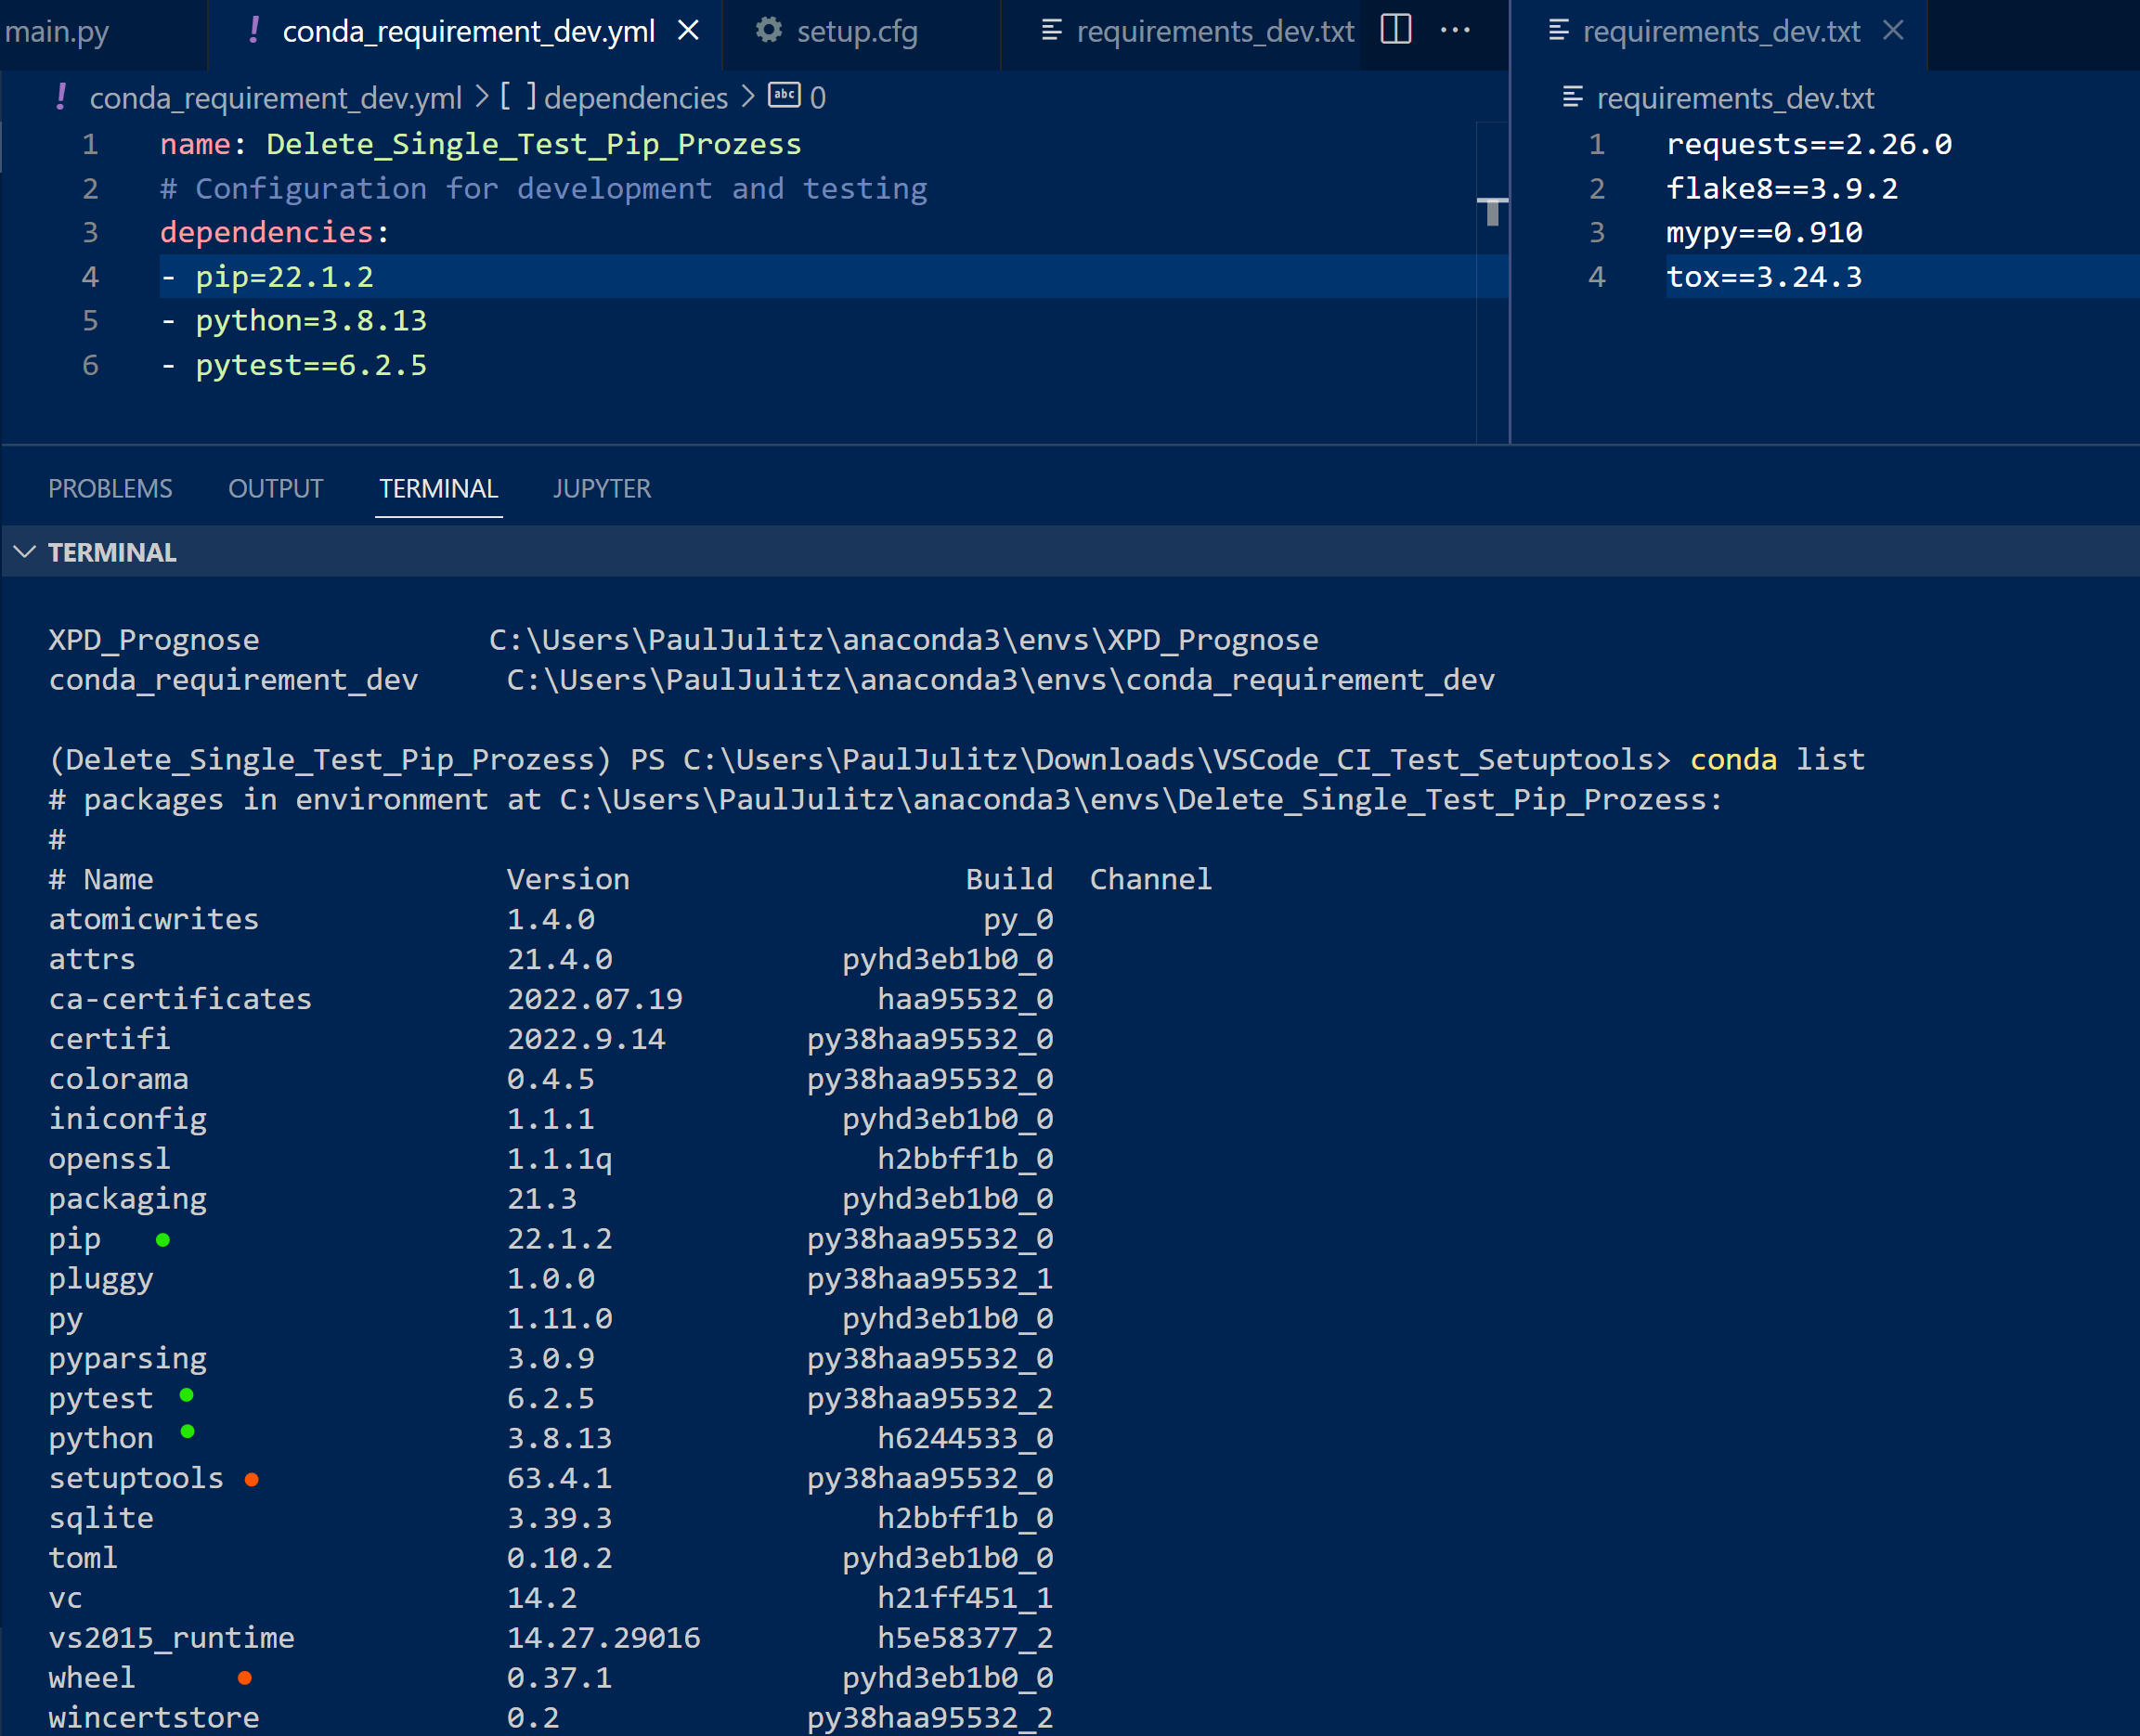
\includegraphics[scale = 0.2]{attachment/chapter_2/Scc084}
	\caption{Bsp für geladenen Pakete der vorherigen requirements Datei}
\end{figure}

Die grünen Punkt zeigen die Pakete, welche direkt über die Requirments Datei angegeben sind. Der Rest der Packet wurde von \gls{g_conda} selbst installiert. Die roten Punkte zeige die Packet welche im weiteren Abschnitten benötigt werden und von \gls{g_conda} mitinstalliert wurden. Es gilt auch hier, wird eine spezifische Versionsnummer benötigt, muss diese über die requirements Datei angegeben werden, sonst wird die aktuelleste Version ausgewählt.\\

Der Befehl 
\begin{lstlisting}[style=Config, caption={Beispiel Nicht übergebener Befehl}, captionpos=b]
	...
	- pip:
	- pip install -e .
\end{lstlisting}

hat nicht über die Initialisierung der Umgebung geklappt. Um setuptools zu starten muss dieser direkt über das Terminal eingeben werden.
%TODO: Test
% Optional; Testen, ob dies wirklich so ist. Vielleicht war der Befehl zu erst falsch, weil  install -r requirments.txt anstatt pip install -r requirments.txt verwendet wurde.


\subsubsection{Conda Befehle}
\begin{itemize}
	\item 
	\begin{lstlisting}[style=CMD]
		conda env create -f <env name>.yml
	\end{lstlisting}
	erstellt ein neue Umgebung. Der Name der Umgebung v on von \textit{<env name>} gesetzt. 
	\item 	\begin{lstlisting}[style=CMD]
		conda list
	\end{lstlisting} gibt alle Packet in der aktiven Umgebung wieder.
	\item 	\begin{lstlisting}[style=CMD]
		conda env list
	\end{lstlisting}  gibt alle lokalen Umgebungen wieder.
	\item 	\begin{lstlisting}[style=CMD]
		conda activate <env name>
	\end{lstlisting}  aktiviert
\end{itemize}

\subsection{Setuptools}
Die Bibliothek \textit{setuptools} hat den Zweck Python Projekte in Bibliotheken umzuwandeln und verteilbare Bibliotheken anzubieten. In dem Abschnitt liegt der Fokus darauf Module aus einem Repository im der eigenen \gls{VEN} zu hinterlegen. Der Mehrwert ist, dass andere Module, welche $"$paralle$"$ zueinander liegen oder eine $"$Ebene$"$ niedriger sortiert sind, auf das Modul im gleichen Repository zugreifen können. \\

Benötigt wird hierfür 
\begin{itemize}
	\item Modul Deklaration: \textit{$\_\_$init$\_\_$.py}
	\item Installationsdatei: \textit{setup.py}
	\item Konfigurationsdateien: \textit{setup.cfg}, \textit{myprojekt.toml}
\end{itemize}

Das Vorgehen wir an einem Beispiel im Folgenden erklärt:
Damit Module innerhalb des Repository gefunden werden können, muss dies deklariert werden. Dies gilt nicht nur für die Hinterlegung in der \gls{VEN}, sonder auch allgemein für den Interpreter.

\begin{figure}[H]
	\centering
	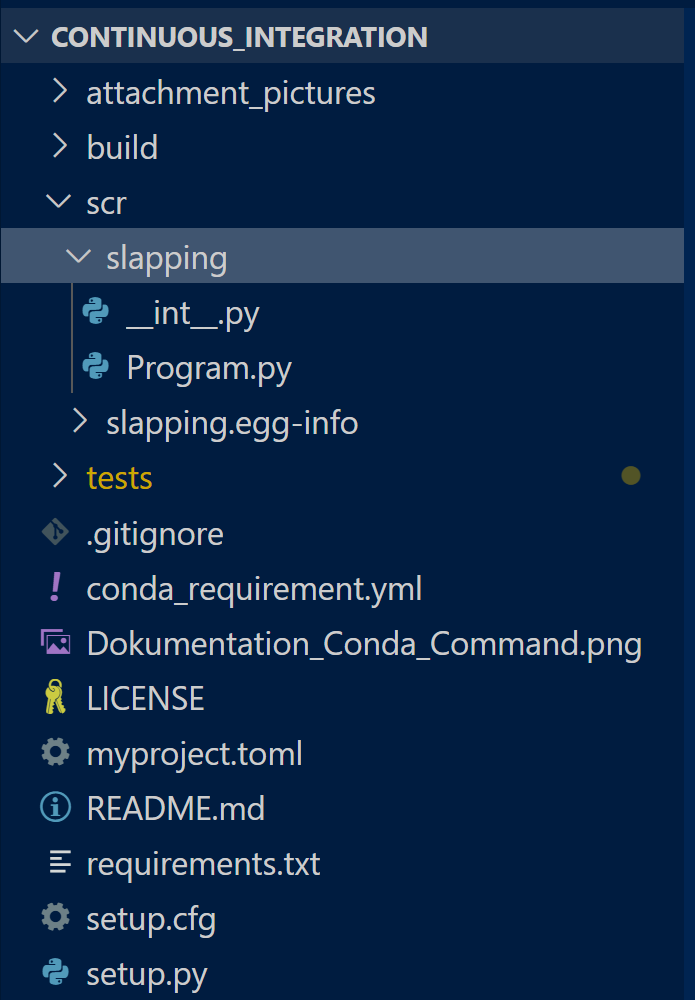
\includegraphics[scale = 0.8]{attachment/chapter_2/Scc070}
	\caption{Bsp.: Slapping Modul}
\end{figure}

Entlang der untere Hierachie kann das Modul jetzt gefunden werden. Das
\begin{itemize}
 \item Installationsdatei: \textit{setup.py}
	\item Konfigurationsdateien: \textit{setup.cfg}, \textit{myprojekt.toml}
\end{itemize} Verzeichnis \textit{test/} kann jedoch die Packete und Module in \textit{scr/} nicht finden.
\begin{figure}[H]
	\centering
	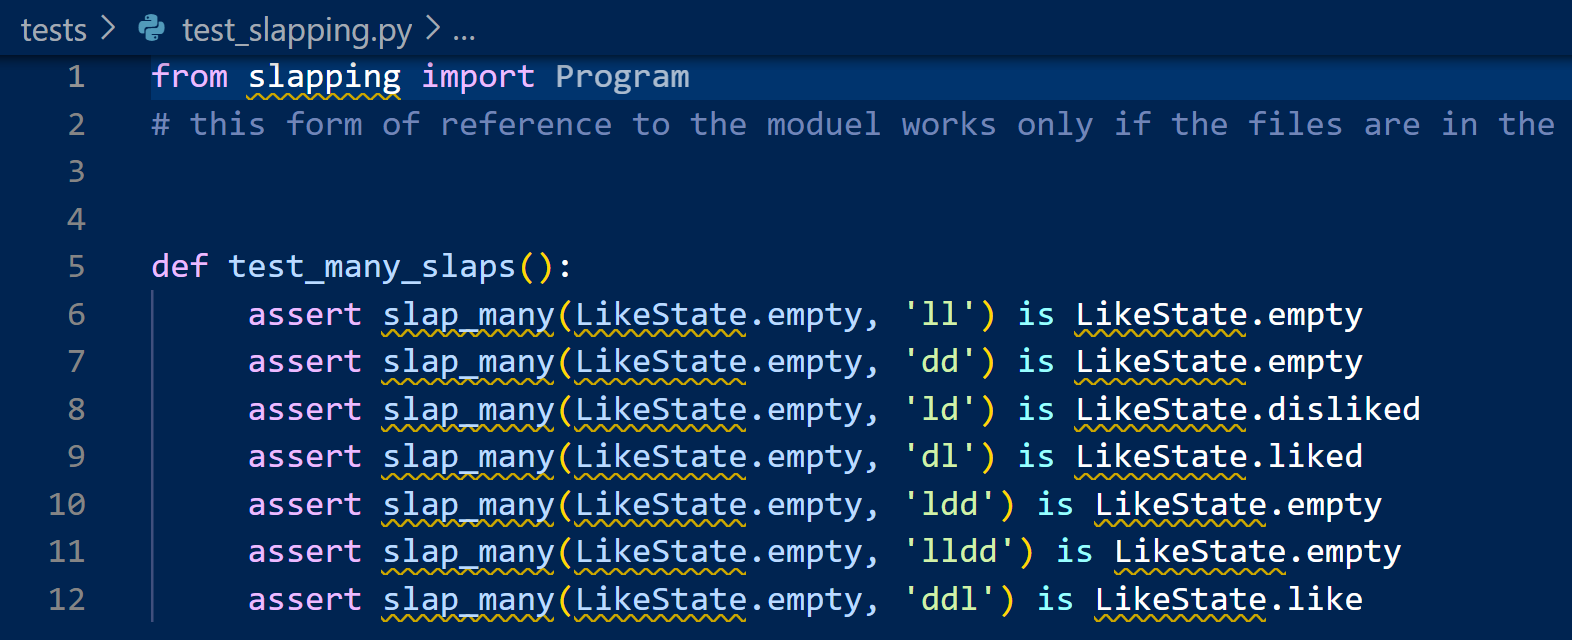
\includegraphics[scale = 0.8]{attachment/chapter_2/Scc071}
	\caption{Bsp.: Problem beim Import im höheren Verzeichnis}
\end{figure}

\subsubsection{2 - Setup.py}
Ein Python Skript mit dem Namen \textit{Setup} wird erstellt. Es können hier ebenso Konfigurationen hinterlegt werden. In dieser Aufführung wird nur \textit{setup()} aus \textit{setuptools} gestartet. \footnote{Aus Sicherheitsgründen wird in diese Datei immer weniger geschrieben. In diesem Fall steht nur der \textit{setup()} Aufruf drin.}
\begin{lstlisting}[style=python]
// setup.py
from setuptools import setup
if __name__ = "__main__":
setup()
\end{lstlisting}

\subsubsection{3 - Konfigurationsdateien}
Wie oben erwähnt, ist in diesem Abschnitt der Fokus darauf, wie Module in die \gls{VEN} hinterlegt/ installiert/ build)\footnote{
	Build is the process, in which source code is converted into a standalone software.
} \footnote{
	\href{https://setuptools.pypa.io/en/latest/userguide/pyproject_config.html}{Quelle}
}

werden können. Die hier beschriebenen Konfigurationsdateien werden unteranderen genutzt, um Test-Bibliotheken zu konfigurieren. Wie die Abwicklung von Test aussieht, wir unter \textit{Automatic Testing} beschrieben.\\

Die Bibliothek, \textit{setuptools}, hat den Standard PEP 621 übernommen, und bezieht die Metadaten für den Build Prozess\footnote{
	Der referierte Source Code ist das Module unter \textit{src}, welche in der \gls{VEN} installiert werden soll. 
} 
aus
\begin{itemize}
	\item \textit{pyproject.toml} und
	\item \textit{setup.cfg}
\end{itemize}
Theoretisch können die Metadaten auch in einer Datei liegen.\footnote{
Die Metadaten für \textit{mypy} und \textit{pytest} werden ebenso unter der toml Datei abgelegt. Für flake8 wird dies in der setup.cfg Datei getan.
}


In der \textit{pyproject.toml} Datei wird wird der \textit{build process} spezifiziert. Diese kann auch wo anderes festgelegt werden, hin dem Bespiel wird der \textit{build process} in der toml Datei festgehalten:
\begin{lstlisting}[style=Config]
[build-system]
requires = ["setuptools>=42.0", "wheel"]
build-backend = "setuptools.build_meta"
\end{lstlisting}

Die Metadaten und Test Packet Konfigurationen wird in \textit{setup.cfg} hinterlegt.
Diese legt neben den Metadaten die Auswahl der eigen gewählten Packete fest. Unter \textit{package} wird festgelegt, wo das Modul sich befindet.

\begin{lstlisting}[style=Config, caption={Beispiel Slapping Modul}, captionpos=b]
	[metadata]
	name = slapping
	...
	[options]
	packages =
	slapping
	install_requires =
	requests>=2
	python_requires = >=3.6
	package_dir =
	=src
	zip_safe = no
\end{lstlisting}

%TODO:STOP
Unter den Optionen für das Modul festgelegt, wo es sich befindet. In dem Beispiel werden auch Requirments festgelegt, welche das Modul besitzen muss. Es wird geprüft, ob diese in der \gls{VEN} vorhanden sind. Ist es nicht, werden die Packet in der neusten Version installiert.\footnote{
	\href{https://setuptools.pypa.io/en/latest/userguide/declarative_config.html}{Quelle Setuptools Guide},
	\href{https://ianhopkinson.org.uk/2022/02/understanding-setup-py-setup-cfg-and-pyproject-toml-in-python/}{Vergleich der Konfigurationsdateien}
}
Sollen mehrere Module installiert werden, so ist dies über setuptools auch möglich. Wird das Verzeichnis mit dem Hauptverzeichnis angegeben, so sucht setuptools nach allen Module. Diese werden als Paket gespeichert. Existiert nur ein Module, besteht das Paket aus einem Modul.\footnote{
	Ob dafür alle Paket Namen angegeben werden müssen, ist unklar.
}


\begin{lstlisting}[style=Config, caption={Setuptools find all packges}, captionpos=b]

# You can set up your setup.cfg to automatically find all your packages in the subdirectory, 
# using package_dir, like this:
# This example contains just the necessary options for a src-layout, set up
# the rest of the file as described above.

[options]
package_dir=
    =src
packages=find:

[options.packages.find]
where=src
\end{lstlisting}



\subsubsection{Installation (Build Process)}
Ist die \gls{VEN} angelegt, wird mit dem Befehl

\begin{lstlisting}[style=CMD]
	pip install -e .
\end{lstlisting}

setuptools aufgerufen. Diese installier das hinterlegte Paket in editierbaren Modus (-e). 
Dies bedeutet, dass ein Link hinterlegt ist, sodass das packet bearbeitet werden kann, ohne dass es neu installiert werden muss.

Ist die Installation erfolgreich abgeschlossen, befindet sich eine Verlinkung des hinterlegten Pakets unter \gls{VEN} wieder. In dem Beispiel \textit{Slapping} ist das Paket \textit{slapping} in der \gls{VEN} hinterlegt.
\begin{figure}[H]
	\centering
	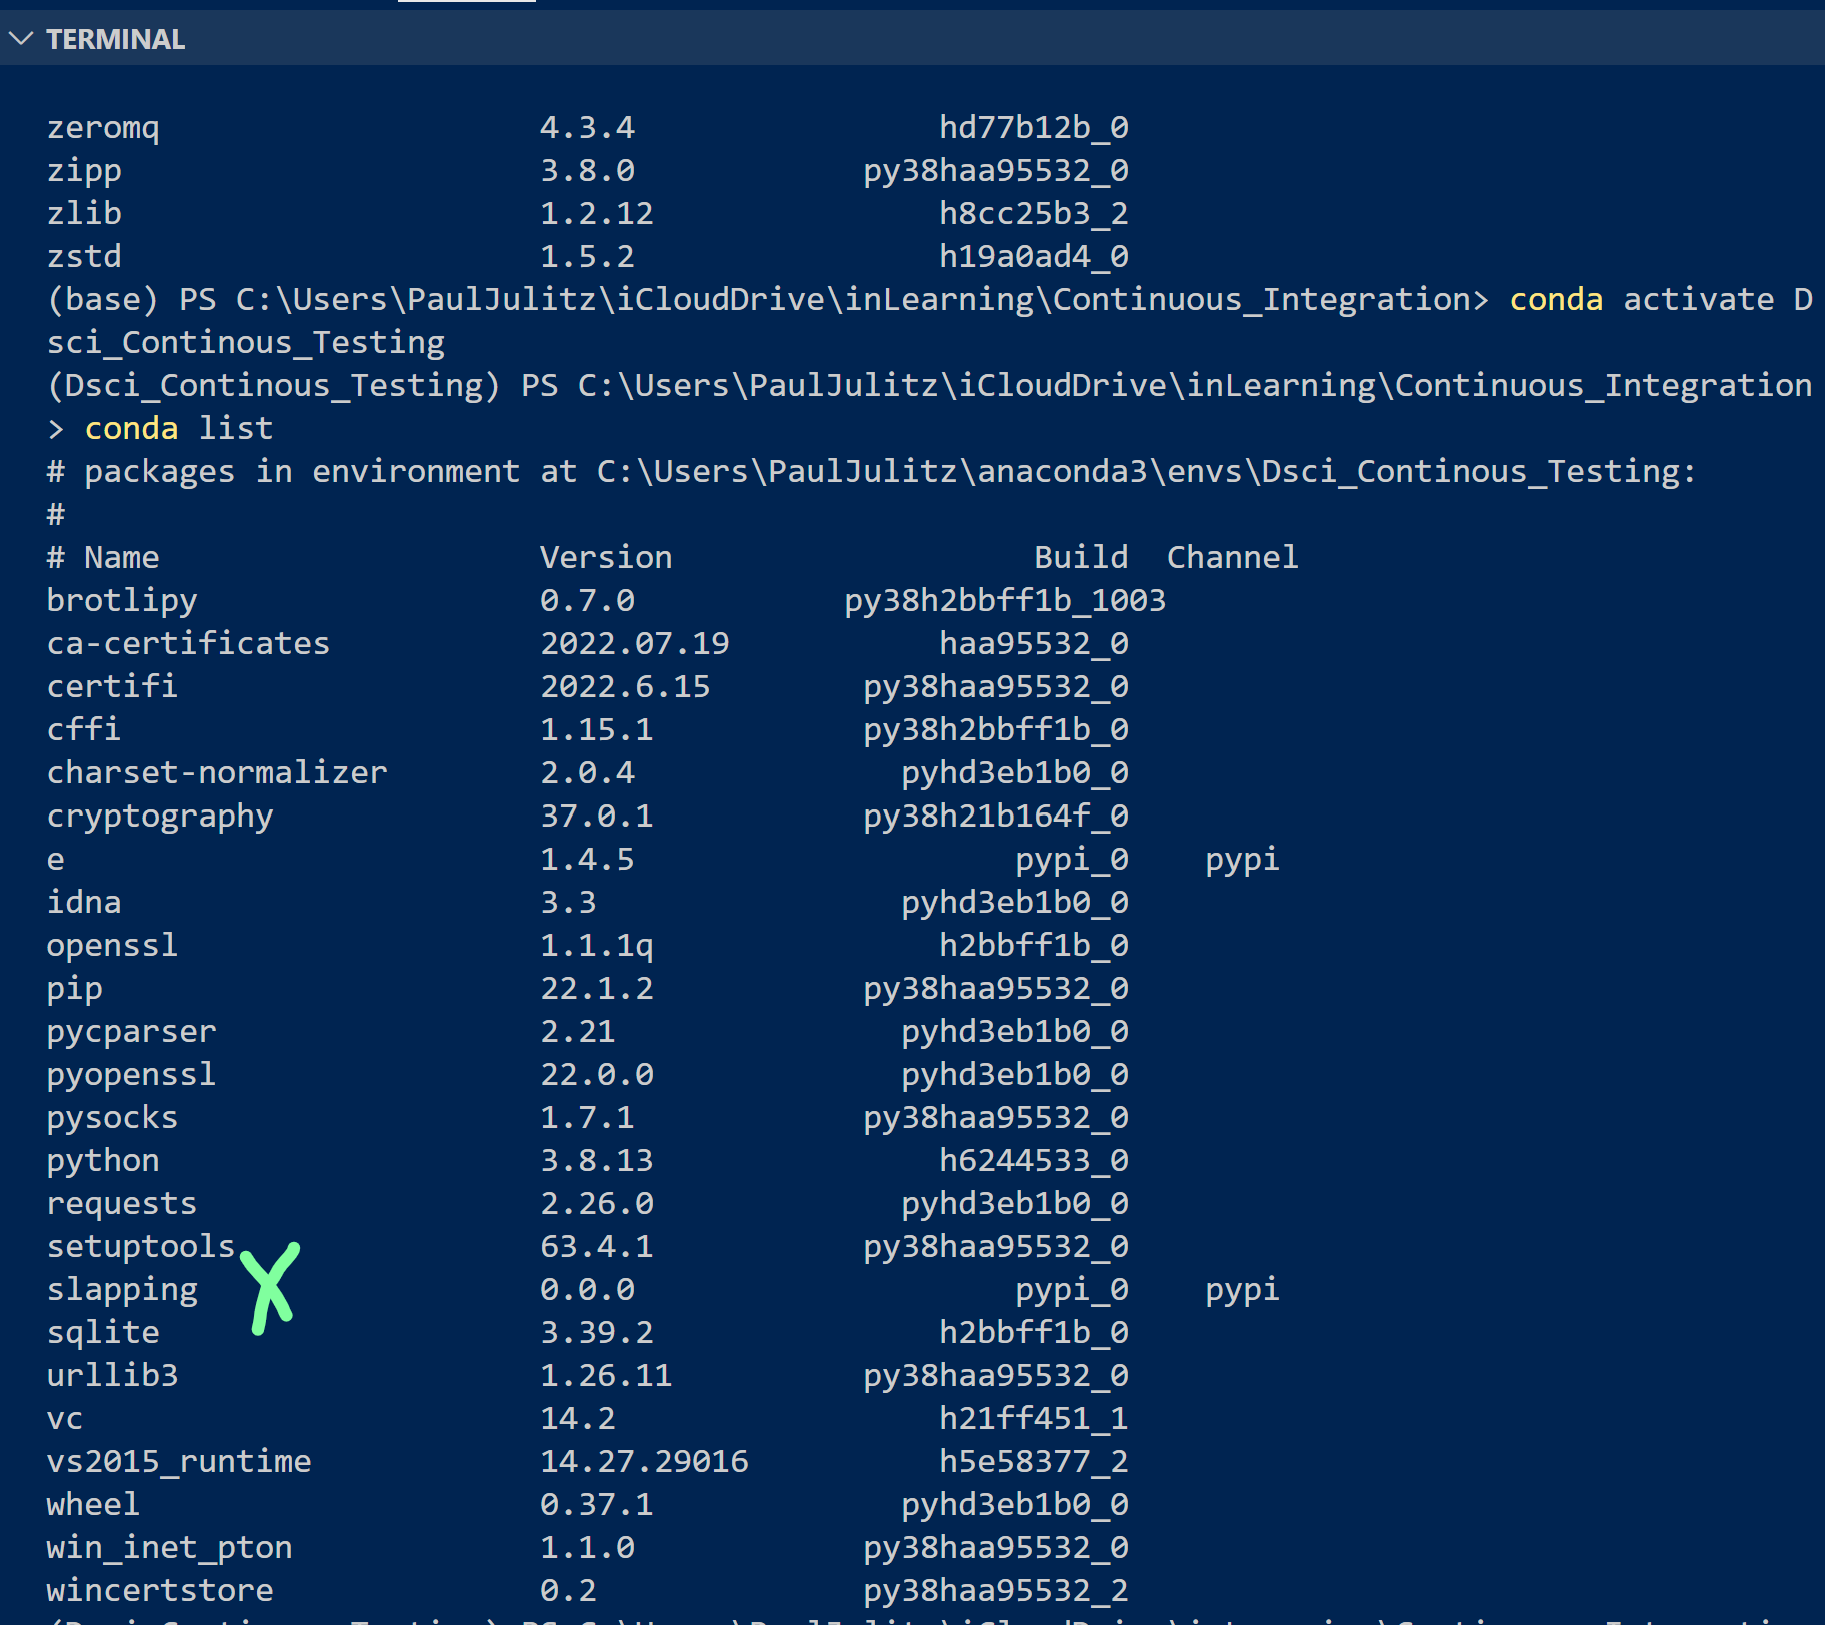
\includegraphics[scale = 0.4]{attachment/chapter_2/Scc074}
\end{figure}

In den Output von setuptools werden die installierten Pakete angezeigt. 
\begin{figure}[H]
	\centering
	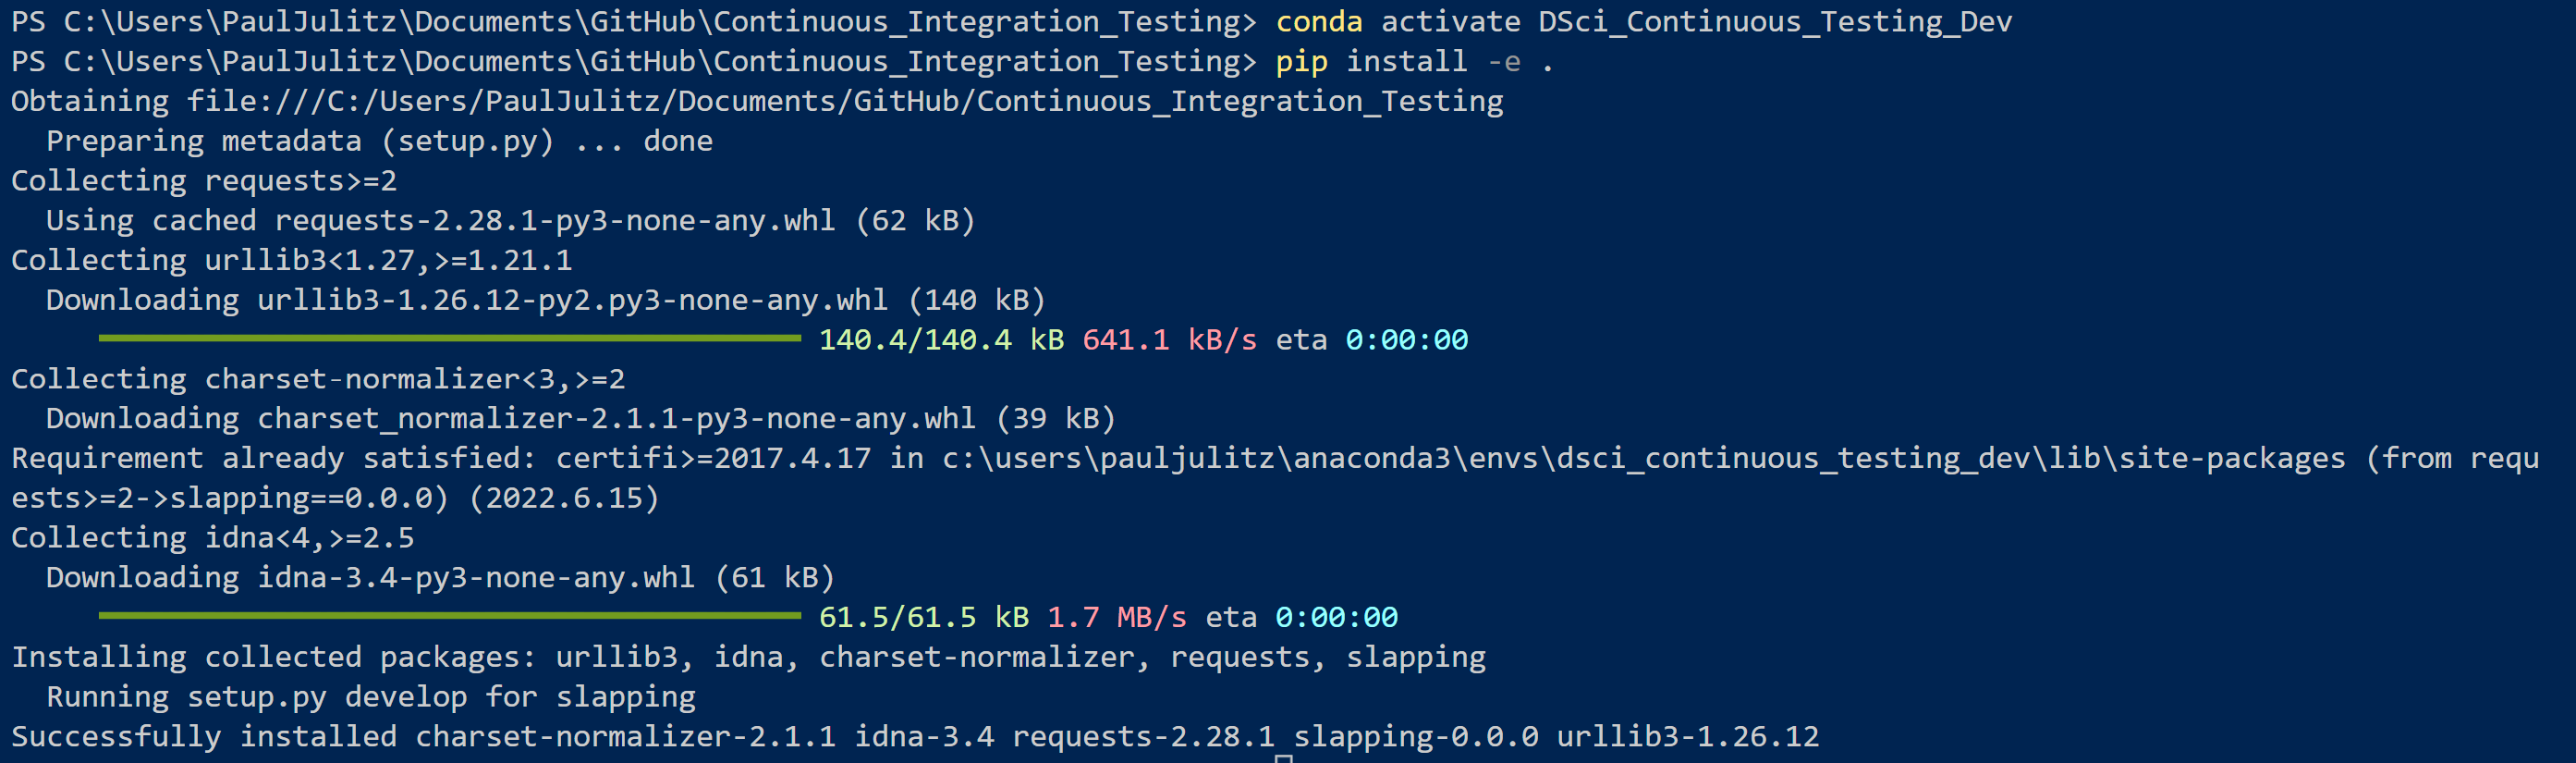
\includegraphics[scale = 0.4]{attachment/chapter_2/Scc076}
\end{figure}
